
\documentclass[%
 reprint,
%superscriptaddress,
%groupedaddress,
%unsortedaddress,
%runinaddress,
%frontmatterverbose, 
%preprint,
%preprintnumbers,
%nofootinbib,
%nobibnotes,
%bibnotes,
 amsmath,amssymb,
 aps,
%pra,
%prb,
%rmp,
%prstab,
%prstper,
%floatfix,
]{revtex4}


\usepackage{dcolumn}% Align table columns on decimal point
\usepackage{bm}% bold math
\usepackage{hyperref}% add hypertext capabilities
\usepackage{graphicx} % Include figure files
\graphicspath{{Figures/}} %Setting the graphicspath

\newcommand{\prior}{{\sc prior}\xspace}
\newcommand{\bilby}{{\sc Bilby}\xspace}
\newcommand{\bilbypipe}{{\sc bilby\_pipe}\xspace}
\newcommand{\bilbypipegdb}{\texttt{bilby\_pipe\_gracedb}\xspace}
\newcommand{\pbilby}{{\sc pBilby}\xspace}
\newcommand{\dynesty}{{\sc dynesty}\xspace}
\newcommand{\cpnest}{{\sc cpnest}\xspace}
\newcommand{\ptemcee}{{\sc ptemcee}\xspace}
\newcommand{\gwpy}{{\sc GWpy}\xspace}
\newcommand{\imrphenomp}{{\sc IMRPhenomPv2}\xspace}
\newcommand{\pycbc}{{\sc PyCBC}\xspace}
\newcommand{\bcr}{{\sc BCR}\xspace}
\newcommand{\pastro}{{$p_\text{astro}$}\xspace}
\newcommand{\msun}{{M${}_\odot$}\xspace}
\begin{document}

\preprint{APS/123-QED}

\title{A Bayesian search to find \\high-mass black holes in LIGO data}% Force line breaks with \\



\author{Author list TBD}

\date{\today}

\begin{abstract}

The detection of high mass black holes ( $>100$ \msun) will shed light on the formation of supermassive black holes and thus galaxy formation. Although LIGO is sensitive to the merger of binary black holes with total masses up to 500 \msun, the largest total mass detected so far is approximately $80$ \msun. A possible explanation for the absence of high mass events may be due to their misclassification as short-duration instrumental noise transients. Short-duration instrumental transients mimic the short-duration gravitational-wave signals from high-mass binary black hole mergers. Here we demonstrate that a new search method utilising Bayesian inference could be a more sensitive tool for detecting high-mass binary black hole mergers as compared to traditional match-filtering. We have applied this technique on the high-mass triggers during LIGO's second observing run to investigate the possibility of discovering new gravitational-wave signals from an entirely new class of high mass black hole binaries.



\end{abstract}

\maketitle

%\tableofcontents


%%%%%%---SECTIONS---%%%%%%%%%%%%
\section{\label{sec:Introduction}Introduction}

Since the 1970s, there has been an accumulation of evidence for stellar-mass and supermassive black holes. In 2019, the Event Horizon Telescope provided the first visual evidence of the supermassive black hole M87  \cite{m87photo}.  As of January 2020, LIGO, Virgo and IAS have confirmed more than a dozen binary black hole systems \cite{GWTC1, IAS0, IAS1, IAS2}. These various discoveries have firmly established the existence of stellar-mass black holes, supermassive black holes and binary black hole systems.  Interestingly, there is still no direct evidence for intermediate-mass black holes, the black holes that lie in between stellar-mass and supermassive black hole systems with masses between $10^2-10^6$ \msun. Thus, the existence of intermediate-mass black holes is still speculative. \\

If intermediate-mass black holes are present, the gravitational waves emitted from the merger of a binary black hole system with at least one intermediate-mass black hole (up to a mass of $400$ \msun) will be detectable by the ground-based gravitational-wave network. Gravitational waves from such systems should occur at a rate of $0-10\text{yr}^{-1}$ \cite{fregeau2006imbhbRatePrediction, mandel2008rates,rodriguez2015bbhRatePredictions}.  However, even after conducting a targeted match-filter based search for gravitational waves from intermediate-mass black holes the largest total mass detected so far is approximately $80$ \msun \cite{salemi2019search, abbott2019gwtc}. A possible explanation for the absence of intermediate-mass events may be due to their misclassification as short-duration instrumental noise transients \cite{blip_glitches}. These glitches can mimic astrophysical signals and hence decrease the significance of true gravitational wave events. 

One method to account for glitches while searching for gravitational waves from coalescing compact binaries is by utilising a signal consistency test \cite{pycbc_short_duration_transients} or a signal coherence test amongst a network of detectors \cite{bci, bcr_paper,  bcr_gw151216, bayesian_odds}. A signal-coherence test such as the Bayesian coherence ratio (\bcr) \cite{bcr_paper} provides a Bayesian odds ratio comparing the probability that the data contains an astrophysical signal versus the probability that the data contains an incoherent glitch or noise. Although an odds ratio, the \bcr can be used  as a frequentistic \textit{ranking statistic}, ranking the likelihood that a trigger is due to a gravitational-wave signal \cite{bcr_paper}. The \bcr as a ranking statistic is much more powerful than a matched-filter SNR as the \bcr incorporates numerous features that may distinguish gravitational waves from noise and demands that signals must be coherent while glitches must be incoherent amongst different detectors. 


In this paper we utilise the \bcr to calculate \pastro, the probability that a signal is of astrophysical origin [cite],  for all the high-mass (systems with total masses in the range of $55-500$ \msun) candidate gravitational-wave signals from compact binary coalescences in the detector data recorded during aLIGO's second observing run (O2).  We find that (a) our search does not identify any new stellar mass or intermediate mass black holes; (b) high-mass events reported in the GWTC-1, including GW170729 (an event with disputed $p_\text{astro}$ amongst various search pipelines) have high \pastro; and that (c) high-mass events detected from independent groups have low \pastro. 


\section{Method}

% PyCBC asks for the 5 citations:
% http://pycbc.org/pycbc/latest/html/credit.html#searches-for-compact-binary-coalescence
Following \citet{bcr_paper}, the \bcr is an odds ratio of the coherent signal hypotheses $mathcal{H_S}$ and the incoherent instrumental feature hypothesis $mathcal{H_I}$. It is given by
\begin{equation}
BCR = \frac{\alpha Z^S}{\Pi^D_{i=1}[\beta Z^G_i + (1-\beta)Z^N_i]}\ .
\end{equation}
The numerator is the probability of obtaining a coherent signal, where $Z^S$ is the evidence for $\mathcal{H_S}$ and $\alpha$ is the prior odds for obtaining a signal $\alpha=P(\mathcal{H_S})/P(\mathcal{H_I})$. The denominator is the probability of obtaining an incoherent glitch or noise amongst the network of $D$ detectors, where $Z_G_i$ and $Z_N_i$ are the evidence for obtaining a glitch in detector $i$ and the evidence for obtaining just noise in detector $i$.

 
We use a Bayesian framework to calculate the \bcr for high-mass candidate events, simulated signal events and  background events (signal-free events ) supplied by the \pycbc \cite{pycbc_code} search in O2  \cite{pycbc_og0, pycbc_og1, pycbc_og2, pycbc_og3, pycbc_og4, pycbc_og5}.  At its core, \pycbc performs a matched-filter search for binary merger signals using a template-bank of gravitational-wave template waveforms to generate triggers. For the trigger to be considered a  candidate event by \pycbc, it must be observed between detectors with the same template and with a time of arrival difference less than the gravitational-wave travel time between detectors \cite{pycbc_og0}. The simulated signal events are artificially created by injecting signals into the detector data. Similarly, \pycbc artificially constructs the background, signal-free, events by applying relative offsets, or time-shifts, between the data of different detectors \cite{pycbc_og0}. 


Figure~\ref{fig:templateBank} depicts the \pycbc template bank, the high-mass search space and the candidate events, simulated events and background events from a one-week stretch of \pycbc's search in O2. 

Week long stretches of analysis because noise-non stationary, glitches will occur at different rates depending on state of detectors 


Dont know the prior odds, 



\begin{itemize}
	\item briefly explain PyCBC search
	\item define triggers
	\item Extract PyCBC foreground, background and software injection trigger's GPS times based on template duration of triggers
	\item analyse the triggers using Bayesian Parameter Estimation to determine $\log{Z_s}$, $\log{Z_g}$ and $\log{Z_n}$
	\item reweight results to account for uncertainties in PSDs
	\item Calculate BCR
	\item Calculate PDFs
	\item Find $\alpha$ and $\beta$ values such that separation of background and software injection PDFs is maximally apart.
	\item use tuned $\alpha$ and $\beta$ from previous step to calculate BCRs for foreground
	\item calculate the $p_{astro}$ of the foreground events to determine the probability of the trigger being from an astrophysical source. 
\end{itemize}


\section{\label{sec:OutlineOfPipelineMethods}Outline of Pipeline Methods}



\section{Significance of a high-mass Bayesian Search}\label{significance}

There are two primary motivations for a targeted high-mass search that utilises Bayesian inference. The first is to help
distinguish gravitational-waves from high-mass systems from noise-transients, and the second is to try to alleviate the
discord in the significance of some of the ``quiet'' gravitational wave events between various search pipelines.

\hypertarget{a-better-detection-statistic}{%
\subsection{A better Detection-statistic}\label{a-better-detection-statistic}}

\hypertarget{gravitational-wave-triggers-and-short-duration-glitches}{%
\subsubsection{Gravitational-wave triggers and short duration glitches}\label{gravitational-wave-triggers-and-short-duration-glitches}}

A foreground trigger is a section of LIGO data identified by data searching pipelines to potentially harbour some
gravitational wave signal (more on triggers in Appendix\textasciitilde\ref{searches}). In the ground-based gravitational wave
detectors, many spurious instrumental noise events fool the pipelines into considering the noise events as triggers
(false-positive triggers). These instrumental-triggers are called glitches. Luckily, unlike triggers from astrophysical
sources, glitches do not often occur at the same time or with the same morphology across the various gravitational wave
detectors -- they are often \emph{incoherent} amongst detectors. Additionally, these short-duration glitches appear very
similar to high-mass gravitational-wave signals, making the two challenging to distinguish. For example, consider
Figure\textasciitilde\ref{fig:compareGlitchAndSignal} that compares a plot of a glitch on the left and a plot of a high-mass GW
candidate on the right.



\begin{figure}

{\centering 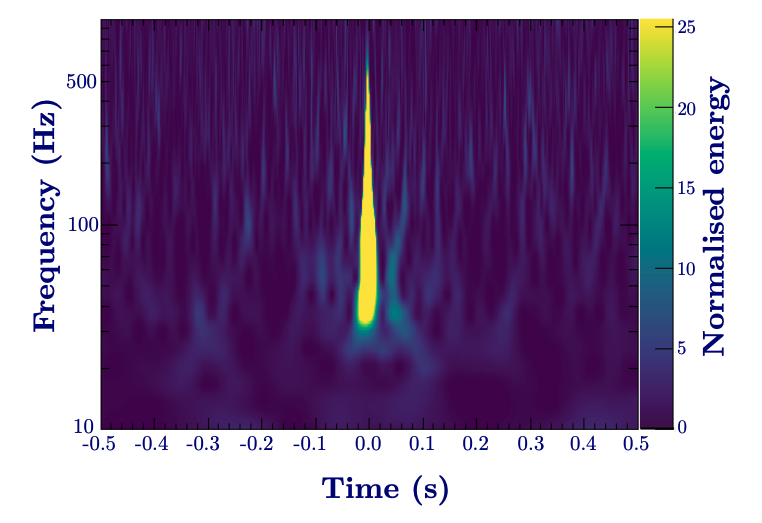
\includegraphics[width=0.45\linewidth]{images/glitch} 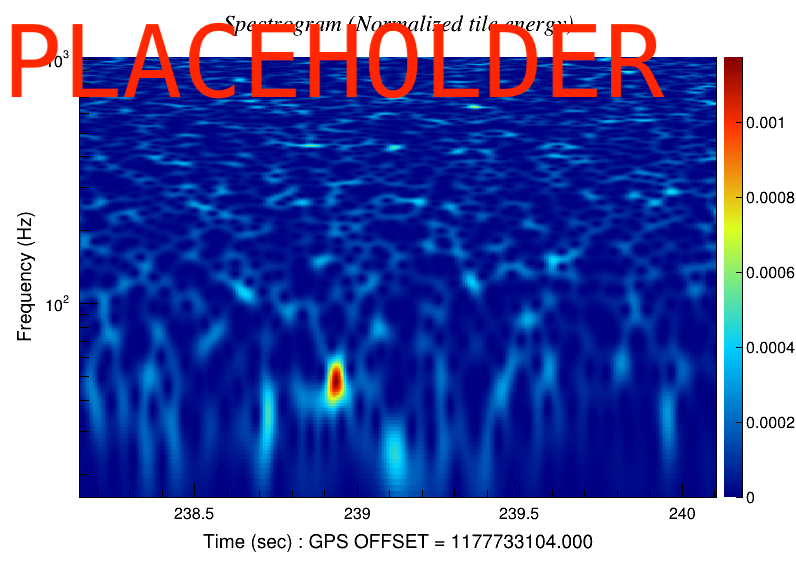
\includegraphics[width=0.45\linewidth]{images/L1_spectrogram_logy_0} 

}

\caption[Comparing glitches to high-mass candidates.]{Spectogram of a glitch on the left, and a candidate GW trigger on the right.}\label{fig:compareGlitchAndSignal}
\end{figure}

\hypertarget{assigning-significance-to-gravitational-wave-triggers}{%
\subsection{Assigning significance to Gravitational-wave triggers}\label{assigning-significance-to-gravitational-wave-triggers}}

The LIGO-Virgo collaboration uses various methods to avoid marking false-positive glitch triggers as gravitational wave
triggers. One method first involves generating a set of \emph{background triggers}, false-positives picked up from the search
through artificially\footnote{The artificial gravitational wave data
  should have no true gravitational waves as it is constructed by applying relative time offsets between the data of different detectors (time offsets longer than the light-travel time between the detectors).} created gravitational
wave data containing no signals. Then, a detection-statistic value, a value
that ranks the likelihood of a trigger to originate from a gravitational-wave signal, is calculated for both the
foreground and background triggers. Finally, the background trigger detection-statistic distribution can assign a probability to the \emph{null hypothesis} that the foreground triggers are consistent with the background. This null hypothesis probability is obtained by first calculating the cumulative distribution function for the background distribution. Placing the foreground event on the background cumulative distribution function provides the \emph{p-value}, or false alarm probability, of the foreground event. This p-value is a measure of how significant indicating the foreground event is from the background distribution of false-positives.

For example, consider the
detection-statistic plot for GW150914, as seen in Figure\textasciitilde\ref{fig:GW150914background}. If the
foreground triggers are far away from the background trigger distribution, the foreground triggers have low p-values (and are significantly
different from the background). Hence, the low p-values foreground triggers might originate from astrophysical sources. On the other hand, if the foreground
triggers fall along with the background distribution with high p-values, the foreground triggers are consistent with the background. Thus,
they are less likely to originate from astrophysical sources.



\begin{figure}[!h]

{\centering 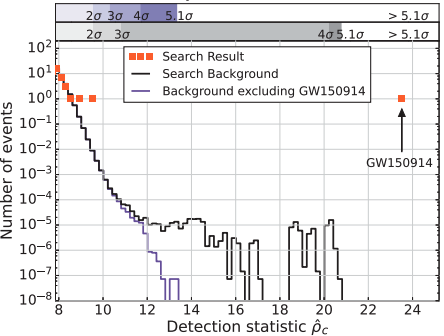
\includegraphics[width=0.75\linewidth]{images/GW150914_background} 

}

\caption[Ranking statistic plot for GW150914]{A binary coalescence search displaying a number of candidate GW events (orange markers) and the mean number of background events (black line), taken from \citet{abbott2016observation}.}\label{fig:GW150914background}
\end{figure}

\hypertarget{a-bayesian-detection-statistic}{%
\subsection{A Bayesian Detection statistic}\label{a-bayesian-detection-statistic}}

Comparing foreground events to a background distribution is a ``frequentist'' method of assigning significance. It does
not use the literal meaning of the likelihood -- which is a probability -- or compute the posterior probability of there
being a signal given data and hypotheses. By using a frequentist method of assigning significance, these searches
discard the physical meaning of the likelihood. In principle, a Bayesian approach would be able to incorporate this
information that is lost.

The goal of this PhD's first project is to enhance the significance of high-mass foreground triggers using a Bayesian
approach and thereby increase the confidence in the detection of gravitational waves from large-mass compact binaries.
If this work does improve the significance of high-mass triggers, we will increase the likelihood of detecting a
high-mass black hole system via gravitational waves. The detection statistic we will utilise is the Bayesian Coherence
Ratio (or BCR), as seen in \citet{bcr_paper}. The BCR is discussed in detail in Appendix\textasciitilde\ref{BayesianCoherenceRatio}. In
short, The \texttt{BCR} is an odds (evidence ratio) comparing two hypotheses: there's a coherent GW in the data, plus Gaussian
noise vs there's only incoherent Gaussian noise or a glitch (modelled as a compact binary coalescence) in each detector
\citep{bcr_paper}.

\hypertarget{a-better-measure-of-significance}{%
\section{A better measure of significance}\label{a-better-measure-of-significance}}

\hypertarget{gravitational-wave-candidates-with-uncertain-significance}{%
\subsection{Gravitational wave candidates with uncertain significance}\label{gravitational-wave-candidates-with-uncertain-significance}}

In aLIGO's first two observing runs, eleven gravitational wave events were found in the data by the LIGO-Virgo
scientific collaboration \citep{abbott2019gwtc}. Since the public release of LIGO's first and second observing run's data,
several groups have searched the data for gravitational waves independently of LIGO. One particular research group of
interest is a research team at the Institute for Advanced Study (IAS). The group constructed searches to look for the
LIGO-confirmed the gravitational wave events detected by the LIGO-Virgo collaboration, and in the process of doing so,
claim to have discovered several others events \citep{IAS0, IAS1, IAS2}. Some of these events have total masses \(>85 M_{\odot}\), which is larger than the average total mass of the LIGO detections. Some of these IAS and LIGO events are
displayed in Table\textasciitilde\ref{tab:O2significancesWObcr} with their p-astro reported by various LIGO and IAS search pipelines.

\begin{table}[t]

\caption[p-astro for various O2 foreground triggers]{\label{tab:O2significancesWObcr}p-astro from several detection pipelines for a subset of the O2 foreground triggers.}
\centering
\begin{tabular}{llrrrr}
\toprule
Event & Catalogue & PyCBC & GstLAL & cWB & IAS\\
\midrule
GW170104 & GWTC-1 & 1.00 & 1.00 & 1.00 & 0.99\\
GW170121 & IAS-1 & NA & NA & NA & 0.99\\
GWC170402 & IAS-2 & NA & 0.09 & NA & 0.68\\
GW170403 & IAS-1 & NA & NA & NA & 0.56\\
IMBHC170423 & IMBH-marginal & NA & 0.00 & 1.00 & NA\\
GW170425 & IAS-1 & NA & NA & NA & 0.77\\
GW170729 & GWTC-1 & 0.52 & 0.98 & 0.94 & NA\\
\end{tabular}
\end{table}

From this Table\textasciitilde\ref{tab:O2significancesWObcr}, it is evident there is some uncertainty if these events can be considered real
gravitational-wave events -- are these events significantly different from the background or not? The various pipelines
have different answers. Our Bayesian search pipeline, as described in the next section, can help us answer this question
and come to a conclusion about the significance of the events.

\hypertarget{using-the-bcr-to-calculate-significance}{%
\subsection{Using the BCR to calculate significance}\label{using-the-bcr-to-calculate-significance}}

While the BCR might not increase the significance of some of the gravitational wave candidates, it will provide a more
accurate measure of their significance. The BCR significance will be more accurate as it is a measure of the probability
that signals in two or more detectors are \emph{coherent} (signals share exactly the same source properties in the different
detectors) vs the detectors having \emph{incoherent} glitches/noise. This Bayesian significance might alleviate the discord
between the significances of specific foreground triggers reported by various search pipelines.

In summary, we will use the BCR to analyse high-mass foreground triggers to help discern signals from glitches and
provide a better measure of significance for the foreground triggers. For our work, we will initially focus on
conducting this BCR search on O2 data, and subsequently with a search in O3 data.


\section{Methodology}\label{methodology}
This PhD project intends to provide new methods and insights to studying gravitational waves form high-mass systems.
Thus far, the project has focused on building up the infrastructure to compare the Bayesian Coherence Ratio of LIGO's
time-shifted \emph{background} triggers, \emph{foreground} triggers and \emph{software injections}. This chapter describes how we have
adapted the methods from \citet{bcr_paper} in our implementation.

\hypertarget{selecting-o3-triggers-for-bcr-analysis}{%
\section{Selecting O3 Triggers for BCR analysis}\label{selecting-o3-triggers-for-bcr-analysis}}

LIGO's third observing run, O3, began on April, 2019, and is going until May 2020 (with a commissioning break during
October). In the 35 observing weeks since O3 started, based off the \(\sim50\) public alerts for gravitational wave
candidate triggers, LIGO might have tripled the number of detections during all of the first and second observing runs,
O1 and O2 \citep{gracedb}. These gravitational wave events are considered candidates, as LIGO is still in the process of vetting the
candidates (making sure that they are from astrophysical sources rather than terrestrial, spurious noise sources). On
top of these candidate triggers, there are numerous sub-threshold triggers (triggers that do not have high
significance).

Ideally, we would like to compute the BCRs for all triggers (foreground and background) produced by LIGO to help improve
the significance of astrophysically real triggers and decrease the significance of glitches. However, computational
limitations prevent analysis of all triggers. Instead, we limit the data to several 8-day chunks from O2, selected based
on the number of foreground triggers identified by \href{https://pycbc.org/}{\texttt{PyCBC}} in the various chunks, as seen in
Figure\textasciitilde\ref{fig:o2TrigCount}. Currently, we are using O2 data as it is public, whereas O3 data is not. By analysing O2
triggers we can publish our results without any restrictions imposed by LIGO.



\begin{figure}[!h]

{\centering 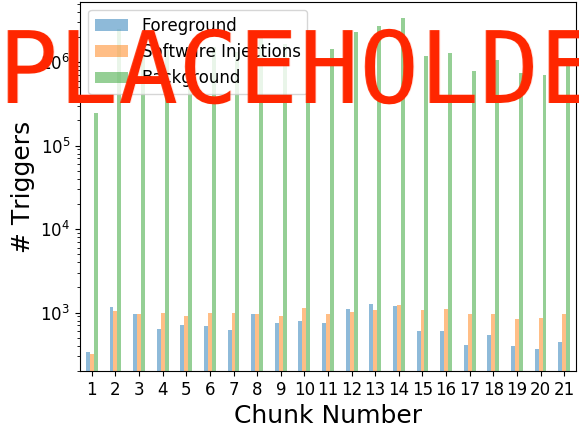
\includegraphics[width=0.75\linewidth]{images/O2_unfiltered_trigger_counts} 

}

\caption[Count of all triggers in PyCBC O2 search]{Counts of triggers from \texttt{PyCBC}'s search through O2 Data (November 15, 2016 - August 26, 2017). Each chunk is roughly 8 days long. The background triggers are collected from timesliding each chunk's data to generate a dataset of roughly 3 million years.}\label{fig:o2TrigCount}
\end{figure}

Additionally, to confine our search to high-mass sources (systems with total masses roughly between 50-500
\(M_{\odot}\)), we restrict the triggers corresponding to a gravitational wave template with durations less than 454 ms.
These short duration templates correspond to compact binary coalesences with the parameters presented in
Table\textasciitilde\ref{tab:parameters} and the search space for these triggers can be visualised in Figure\textasciitilde\ref{fig:templateBank}.

\begin{table}[t]

\caption[BBH parameters corresponding to durations $<454$ ms]{\label{tab:parameters}Template Banks's parameters for templates with duration $<454$ ms.}
\centering
\begin{tabular}{lrr}
\toprule
  & Minimum & Maximum\\
\midrule
Component Mass 1 $[\text{M}_{\odot}]$ & 31.54 & 491.68\\
Component Mass 2 $[\text{M}_{\odot}]$ & 1.32 & 121.01\\
Total Mass $[\text{M}_{\odot}]$ & 56.93 & 496.72\\
Chirp Mass $[\text{M}_{\odot}]$ & 8.00 & 174.56\\
Mass Ratio & 0.01 & 0.98\\
\end{tabular}
\end{table}



\begin{figure}[!h]

{\centering 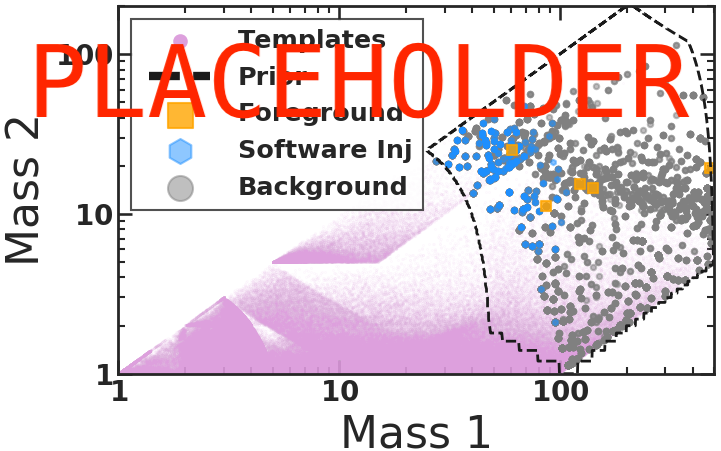
\includegraphics[width=0.75\linewidth]{images/template_bank_masses} 

}

\caption[High-mass BCR search space.]{The template bank used by \href{https://pycbc.org/}{\texttt{PyCBC}} to search in O2's chunk 14. Our search is constrained to the high-mass parameter space enclosed by the dashed line (triggers with duration \(<45s\).}\label{fig:templateBank}
\end{figure}

By restricting the \href{https://pycbc.org/}{\texttt{PyCBC}} triggers only based on the template duration, we acquire common (high FAR) and rare (low
FAR) triggers. It would be straightforward in principle to broaden our template-duration constraint to encompass all
triggers produced by all the various search pipelines. However, we refrain from doing so to keep our computational costs
manageable. A plot of the counts of the triggers in O2 after down-sampling the triggers based on the template duration
can be viewed in Figure\textasciitilde\ref{fig:o2FilteredTrigCount}.



\begin{figure}[!h]

{\centering 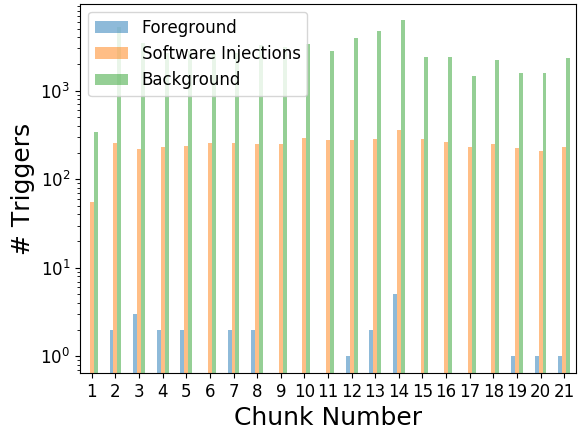
\includegraphics[width=0.75\linewidth]{images/O2_filtered_trigger_counts} 

}

\caption[Count of triggers in PyCBC O2 search shorter than 454 ms]{Counts of triggers from \texttt{PyCBC}'s search through O2 Data, filtered to include only the triggers with a duration less than 454 ms}\label{fig:o2FilteredTrigCount}
\end{figure}

\hypertarget{bcr-analysis-procedure}{%
\section{BCR Analysis Procedure}\label{bcr-analysis-procedure}}

\hypertarget{computational-setup}{%
\subsection{Computational setup}\label{computational-setup}}

To compute the evidence making up the BCR (described in Section\textasciitilde\ref{bcrCalculation}), we use \href{https://lscsoft.docs.ligo.org/bilby_pipe/}{\texttt{bilby\_pipe}} to acquire
the LIGO data in 4s-long data segments containing each trigger (analysis segments) and run the nested-sampling algorithm
implemented in the \texttt{dynesty} library. We utilise \href{https://lscsoft.docs.ligo.org/bilby_pipe/}{\texttt{bilby\_pipe}} to generate PSDs via Welch's method for each data
segment by taking 128 seconds of the data before the analysis segment. If the data quality is not marked as `Science
Mode' for either the PSD or analysis data, then the analysis of that trigger is skipped. Gravitational-wave templates
are produced using \texttt{IMRPhenomPv2} \footnote{\texttt{IMRPhenomPv2} is a standard phenomenological waveform model constructed in the
  frequency domain that models the inspiral, merger, and ringdown (IMR) of a compact binary coalescence with aligned spins
  \citep{khan2016frequency}.}. Although gravitational wave templates that are created from numerical relativity simulations
incorporate more physics than \texttt{IMRPhenomPv2}, we still use this waveform as it is faster to evaluate than numerical
relativity models.

\hypertarget{bayesian-parameter-estimation}{%
\subsection{Bayesian Parameter Estimation}\label{bayesian-parameter-estimation}}

We restrict the priors for Bayesian parameter estimation on the masses such that we only consider signals that are less
than 454ms in duration, as presented in Table\textasciitilde\ref{tab:parameters}. The spins are set to be aligned with a range from
{[}0,1{]}. The prior on luminosity distance assigns probability uniformly in comoving volume, with an upper cutoff of 5 Gpc.
The \href{https://pycbc.org/}{\texttt{PyCBC}} search that originally produced our set of triggers considered a more comprehensive range of masses and
spins than we do in the BCR computation for this project. To accommodate this, we screened the triggers to only allow
triggers with masses within our priors. The run time on a single trigger using the \href{https://arxiv.org/abs/1904.02180}{\texttt{dynesty}} implementation of nested
sampling, with \(2,000\) live points and \(100\) walkers is usually between \(0.5-12\) hours (where the speed often depends on
the SNR of the data segment).

\hypertarget{bcrCalculation}{%
\subsection{BCR calculation}\label{bcrCalculation}}

The Bayesian coherence ratio (BCR), as seen in \citet{bcr_paper}, is the odds between the hypothesis that the data comprise a
coherent, compact binary coalescence signal in Gaussian noise (\(\mathcal{H}_S\)), and the hypothesis that they instead
comprise incoherent instrumental features (\(\mathcal{H}_I\))---meaning each detector has either a glitch in Gaussian noise
(\(\mathcal{H}_N\)) or pure Gaussian noise (\(\mathcal{H}_G\)). For a network of \(D\) detectors,

\begin{equation}
\mathrm{BCR} = \frac{\alpha Z^{S}}{\prod_{i=1}^{D}\left[\beta Z_{i}^{G}+(1-\beta) Z_{i}^{N}\right]}\ , \label{eq:bcr}
\end{equation}
where \(Z^S\) is the evidence for \(\mathcal{H}_S\), and \(Z^{G}_i\) and
\(Z^N_i\) are the evidences for \(\mathcal{H}_{Gi}\) and \(\mathcal{H}_{Ni}\),
in the \(i^{\text{th}}\) detectors. The arbitrary weights \(\alpha\) and \(\beta\)
parametrise our prior belief in each model:

\begin{itemize}
\item
  \(\alpha = P(\mathcal{H}_S)/P(\mathcal{H}_I)\)
\item
  \(\beta = P(\mathcal{H}_{Gi}|\mathcal{H}_I)=1-P(\mathcal{H}_{N}|\mathcal{H}_I)\)
\end{itemize}

for all \(i\) detectors. As most of the data should be noise, we expect both \(\alpha\) and \(\beta\), to be less than 1.
These parameters will be tuned to minimise the overlap between the signal and noise trigger populations.

\hypertarget{trigger-sets-for-bcr-analysis}{%
\subsection{Trigger sets for BCR analysis}\label{trigger-sets-for-bcr-analysis}}

We calculate the BCRs using the procedure described above for three separate trigger sets: background triggers,
foreground triggers, and software injections. The software injections created using masses, spins and distances that
span our priors. The software injections are inserted in the O2 data from where the other triggers are retrieved.

We expect the background trigger BCRs to favour the incoherent glitch hypothesis, and the software injection BCRs to
favour the coherent, compact binary coalescence hypothesis. The foreground trigger BCRs should fall along with the
background if the foreground trigger is a glitch, and with the software injections if the foreground trigger is a
gravitational wave candidate. For example, consider Figure\textasciitilde\ref{fig:bcrIfar} that contains a plot of the BCRs for
several O1 background triggers, foreground triggers, and software injections plotted against iFAR (inverse
false-alarm-rate). In the figure, some foreground triggers fall along the background distribution, these are discarded
as glitches. The foreground triggers that fall along the bulk of software injections are considered gravitational wave
candidates.



\begin{figure}[!h]

{\centering 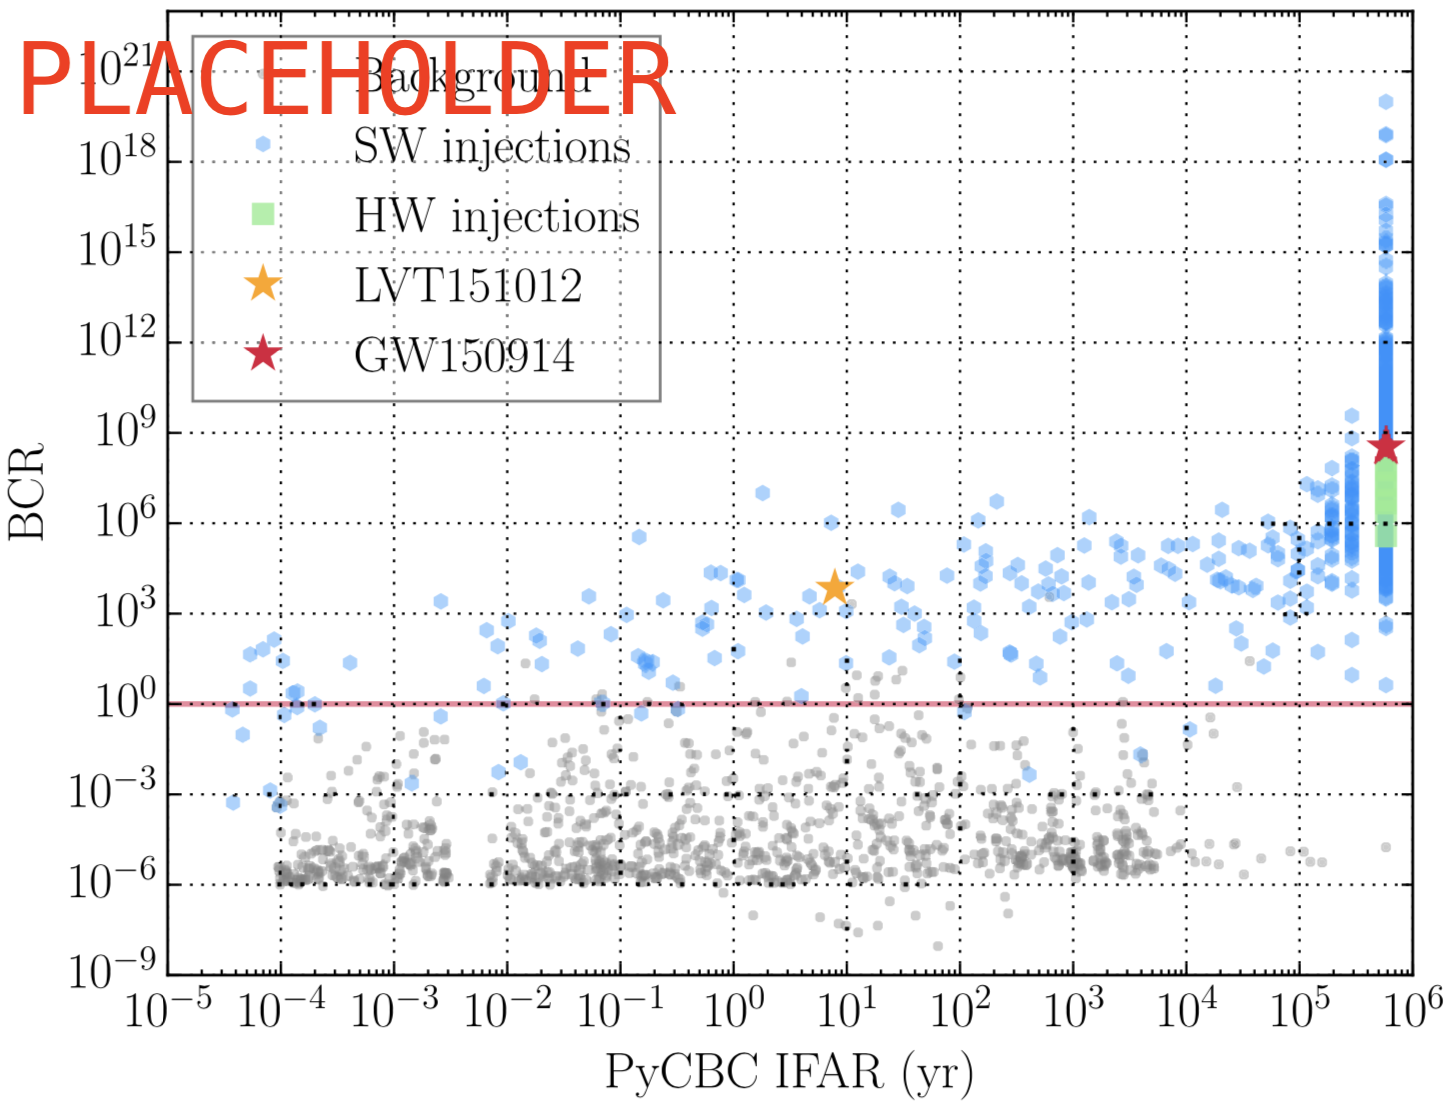
\includegraphics[width=0.75\linewidth]{images/bcr_ifar} 

}

\caption[BCR vs iFAR for O1]{BCR versus iFAR distributions from simulated signals (blue), hardware injections (green), GW events (stars) and background triggers (black), taken from \citet{bcr_paper}.}\label{fig:bcrIfar}
\end{figure}

\hypertarget{making-a-significance-statement}{%
\subsection{Making a significance statement}\label{making-a-significance-statement}}

After obtaining the BCRs for the foreground triggers, background triggers, and software injections, we can make a
statement about the significance of foreground events. For example, consider Figure\textasciitilde\ref{fig:bcrCdf} which displays ln
BCR distributions obtained from our BCR pipeline for aLIGO O2 PyCBC chunk three background triggers and software injections.
The figure also displays the ln BCR values obtained for four foreground triggers. The two foreground triggers with low
ln BCRs are confirmed glitches. The rightmost foreground trigger is GW170104, a gravitational wave event confirmed by
LIGO, and shows much stronger evidence for it being a coherent, compact binary coalescence signal, rather than it being
an incoherent glitch. The remaining foreground trigger corresponds to a gravitational wave candidate identified by the
IAS group.



\begin{figure}[!h]

{\centering 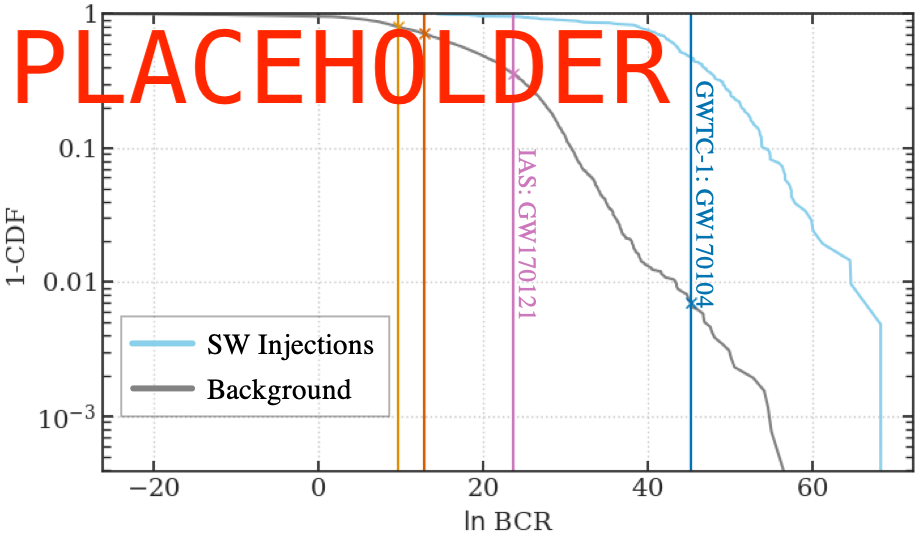
\includegraphics[width=0.75\linewidth]{images/bcr_cdf} 

}

\caption[BCR distribution example]{Histograms represent the survival function (1-CDF) from our selection of 2407 aLIGO O2 PyCBC chunk 3 background triggers (gray) and 648 simulated signals (blue). Vertical lines mark the ln BCRs of two glitches (orange and yellow), IAS's GW170121 (pink), and GWTC-1's GW170104 (dark blue).}\label{fig:bcrCdf}
\end{figure}

Irrespective of the BCR's Bayesian interpretation, we may treat the BCR as a traditional detection statistic to obtain a
frequentist estimate of the significance of any given foreground event based on the measured background with a p-value.
The p-value of foreground events can be obtained from the background's survival function. For example, in
Figure\textasciitilde\ref{fig:bcrCdf}, the p-value for GW170104 is 0.99, denoting that it is significantly different from the bulk
of the background distribution and hence likely to have astrophysical origins. On the other hand, the p-value for the
IAS candidate is 0.65, demonstrating that this candidate might be a glitch.

To calculate the p-value, we need first to calculate fits to the BCR probability
distributions and then tune the BCR's parameters. The following subsections describe these calculations.

\hypertarget{fitting-bcr-data}{%
\subsubsection{Fitting BCR data}\label{fitting-bcr-data}}

Although the BCR should favour the coherent signal hypothesis for software injections,
software injections with a very low SNR might not look coherent amongst an ensemble of
detectors. Hence, software injections are likely to have two probability distributions
of BCRs, one probability distribution of low BCRs corresponding to the software
injections that have very low SNRs and another probability distribution of software
injections with high BCRs. Due to this, we use Gaussian mixture models with two Gaussian
components to fit our BCR distributions.

\hypertarget{tuning-of-bcr-using-kl-distance}{%
\subsubsection{Tuning of BCR using KL Distance}\label{tuning-of-bcr-using-kl-distance}}

The BCR has two tunable parameters as described in Section\textasciitilde\ref{bcrCalculation},
\(\alpha\) and \(\beta\). Altering \(\alpha\) translates the BCR probability distributions for
the triggers while adjusting \(\beta\) spreads the probability distributions out. Although
Bayesian hyper-parameter estimation might be able to determine the optimal values for
these parameters, an easier approach is to manually adjust the parameters for each data
chunk's BCR distribution. In this study, we manually adjust \(\alpha\) and \(\beta\) to
maximally separate the BCR distributions for the software injections and background
triggers.

To calculate the separation between the background and software injection BCR
distributions, we use the Kullback--Leibler divergence (also called relative entropy, or
KL divergence) to quantify how different how the background and software injection BCR
probability distributions are. If the distributions are identical, the KL divergence is
equal to 0, and the KL divergence increases as the asymmetry between the distributions
increases. Figure\textasciitilde\ref{fig:klDivGrid} displays a contour plot of O2 Chunk 14's KL
divergences between the background and software injection triggers for values of
\(\alpha\) and \(\beta\) ranging from \(1^{-10}\) to \(1\). We select these ranges for \(\alpha\)
and \(\beta\) as values outside this range will not make physical sense. Note that for a
fixed value of \(\beta\), the KL divergence stays the same as we alter \(\alpha\). This is
because \(\alpha\) translates the BCR values, but does not alter the distributions
themselves.



\begin{figure}[!h]

{\centering 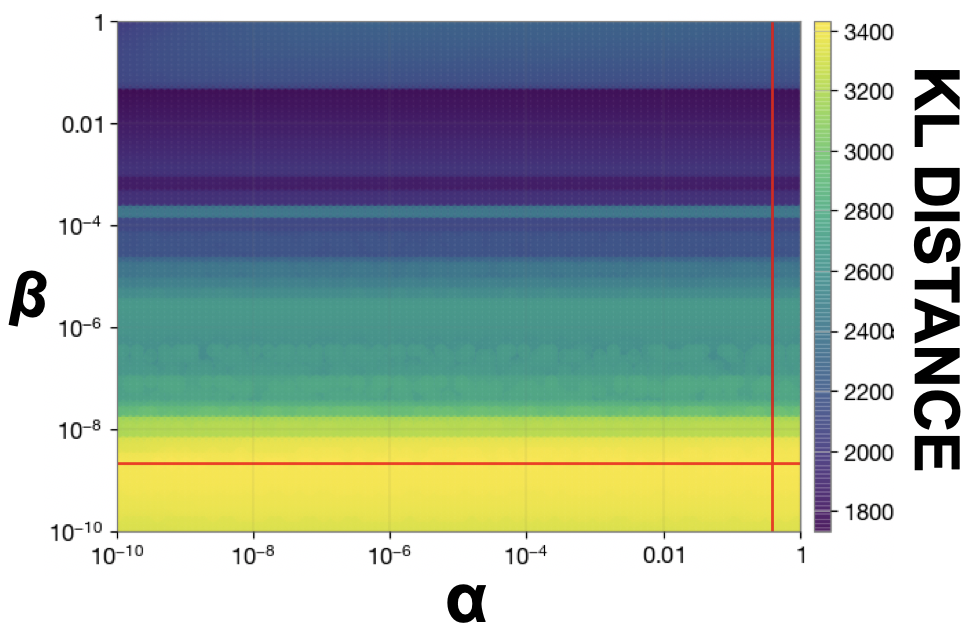
\includegraphics[width=0.75\linewidth]{images/kl_divergence_grid} 

}

\caption[KL Divergence grid for both BCR tunable parameters]{KL Divergences for O2 Chunk 14's software injection and background trigger BCR probability distributions. The red line indicates the \(\alpha\) and \(\beta\) parameters with the maximum KL divergence in this range of \(\alpha\) and \(\beta\).}\label{fig:klDivGrid}
\end{figure}

Figure\textasciitilde\ref{fig:klDivLine} displays a plot of O2 Chunk 14's KL divergences only as
\(\beta\) is adjusted for a fixed \(alpha=1^{-6}\). The \(\alpha\) and \(\beta\) are then selected
based on the combination that results with the maximum KL divergence.



\begin{figure}[!h]

{\centering 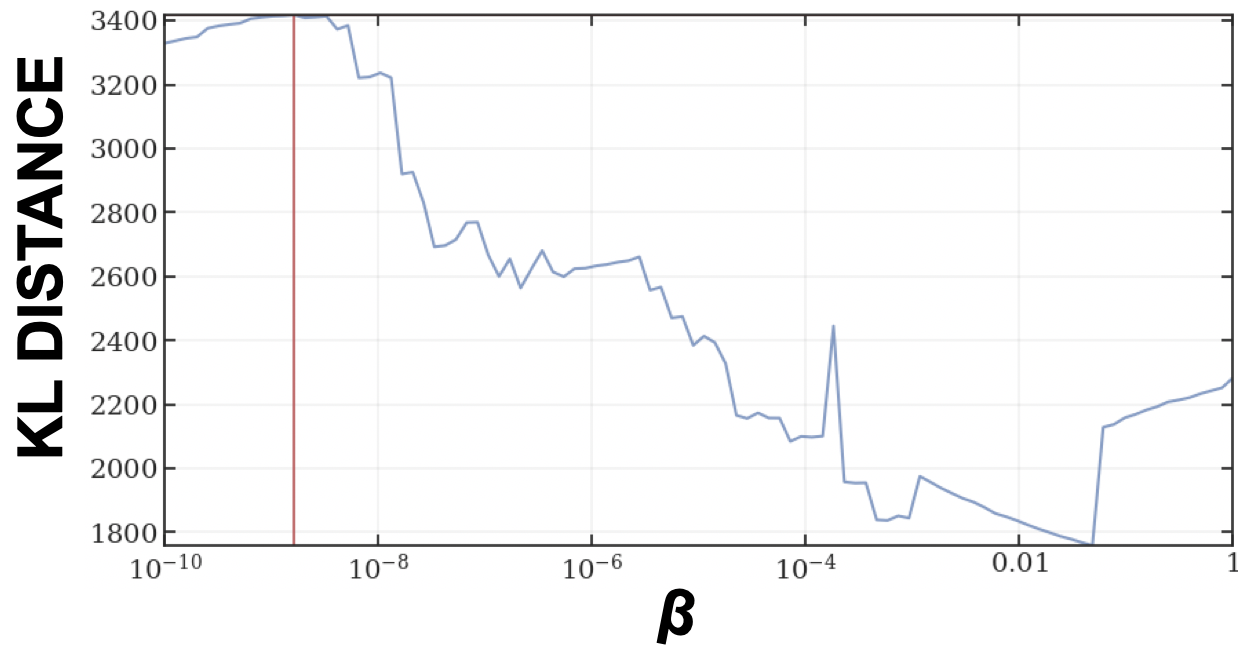
\includegraphics[width=0.75\linewidth]{images/kl_distance_14} 

}

\caption[KL Divergences for one BCR tunable parameter]{KL Divergences for O2 Chunk 14's software injection and background trigger BCR probability distributions with \(alpha=1^{-6}\).}\label{fig:klDivLine}
\end{figure}

In Chapter\textasciitilde\ref{progress} we present some of the preliminary BCR search results we
have obtained from the analysis of various O2 data chunks.




\section{\label{sec:Analysis}O2 Sub-threshold Event Analysis}
\hyperlink{https://docs.google.com/spreadsheets/d/1hm7lFsYneY8NGbFDr-vH5YYsILrxcTexO9D1AvF1qJo/edit?usp=sharing}{Important triggers spreadsheet}
\begin{itemize}
    \item BCRs of O2 sub-threshold high mass events
    \item BCRs of Princeton group's high-mass  events
\end{itemize}


\section{\label{sec:Conclusion}Conclusion}
The detection of high mass black holes (\(>100\) M\({}_\odot\)) will shed light on the formation of globular clusters,
supermassive black holes and thus galaxy formation \citep{lodato2006supermassive, 2018IMBHreview}. LIGO is theoretically
sensitive to the merger of binary black holes with total masses up to 500 M\({}_\odot\) which are expected to occur at a
rate of 0-10 yr\(^{-1}\) \citep[\citet{mandel2008rates}]{fregeau2006imbhbRatePrediction}. However, even after \citet{salemi2019search}'s
targeted match-filter based search for gravitational waves from high-mass black holes the largest total mass detected so
far is approximately 80 M\({}_\odot\) \citep{abbott2019gwtc}. A possible explanation for the absence of high mass events may be
due to their misclassification as short-duration instrumental noise transients \citep{blipGlitches}. High-mass mergers have
very few in-band wave cycles, and hence can easily be mistaken for short-duration instrumental transients. More details
on the theorised formation channels and merger rates are discussed in Appendix \ref{literature}.

We start by developing a targeted search for gravitational waves from high-mass black hole systems. This new targeted
search utilises Bayesian inference and thus is a more sensitive tool for detecting high-mass binary black hole mergers
as compared to traditional match-filtering searches. We have applied this technique on the high-mass triggers during
LIGO's second observing run to investigate the possibility of discovering new gravitational-wave signals from an
entirely new class of high mass black hole binaries.
%%%%%%---SECTIONS-END---%%%%%%%%%%%%

%%%%%%---ACKNOWLEDGEMENTS---%%%%%%%%%%%%
\begin{acknowledgments}
Helpful comments, OzGrav, LIGO, NSF

\end{acknowledgments}
%%%%%%%%%%%%%%%%%%%%%%%%

%%%%%%%%%%%%%%%%%%%%%%%%
\appendix
\section{Appendixes}
%%%%%%%%%%%%%%%%%%%%%%%%


\bibliography{high_mass_bib}% Produces the bibliography via BibTeX.

\end{document}
%
% ****** End of file apssamp.tex ******
